\section{Mechanik}
\label{sec:Mechanik}

% #TODO: Abschnitt kontrollieren
% #TODO: Abschnitt final absegnen (erst wenn alles andere auch fertig ist!)

% #TODO: Bilder mit Pfeilen und Text versehen

% Wie ist das System realisiert?

\begin{wrapfigure}{r}{0.55\textwidth}
    \centering
    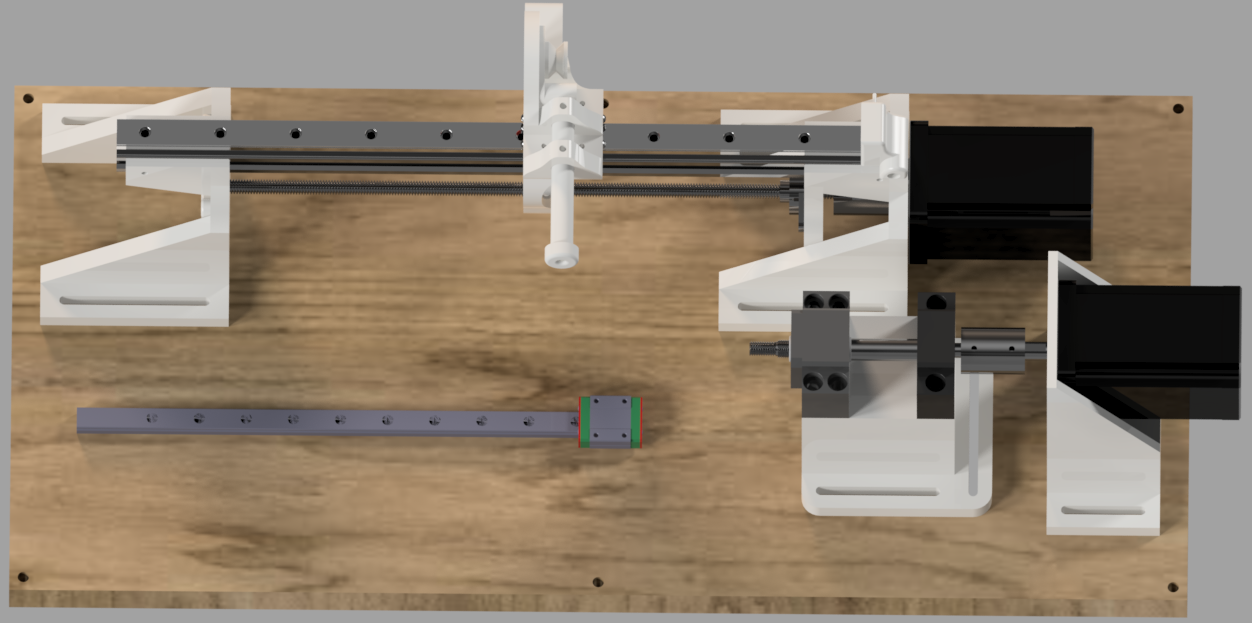
\includegraphics[width=0.55\textwidth]{./winder_render.png}
\end{wrapfigure}

Aufgeteilt ist das Projekt in zwei mechanische Untersyteme, das Drahtspannsystem und der Winder.
Beide Systeme wurden mit 3D-Druck-Teilen aus PETG und Frästeilen aus MDF gebaut und mithilfe unterschiedlicher Schraubsysteme verbunden. Mit Ausnahme der Kaufteile und des Aufnahmewelle, welcher aus hochfestem Stahl passgenau gedreht wurde.



Der Winder besteht aus einer reinen Drehachsen, sowie einem Lineartisch mit gekoppelter Trapetzspindel. Beide Achsen werden jeweils durch einen Steppermotor bewegt. Für die Spulenwicklung, wird der Spulenkörper am Linksgewinde der Aufnahmewelle befestigt und die Achse vom Motor im Uhrzeigersinn gedreht. Die Trapetzspindel kann hingegen in beide Richtungen gedreht werden, bzw. der Lineartisch in beide Richtungen fahren, wodurch die Position des, durch den am Tisch befestigten Aufnahmedorn laufenden, Drahtes, relativ zum Spulenkörper, verändert werden kann. Des Weiteren ist am Lineartisch ein Rotary-Encoder verbaut, sowie ein Gleitlager zur Drahtführung. Sowohl die Gleitlagerhalterung nahe dem Encoder, als auch der Aufnahmedorn, enthalten im Inneren einen Einsatz aus Teflon, um die Reibung zwischen Draht und Führung klein zu halten und Abreibung der Drahtisolation zu vermeiden.

% \begin{figure}[H]
%     \centering
%     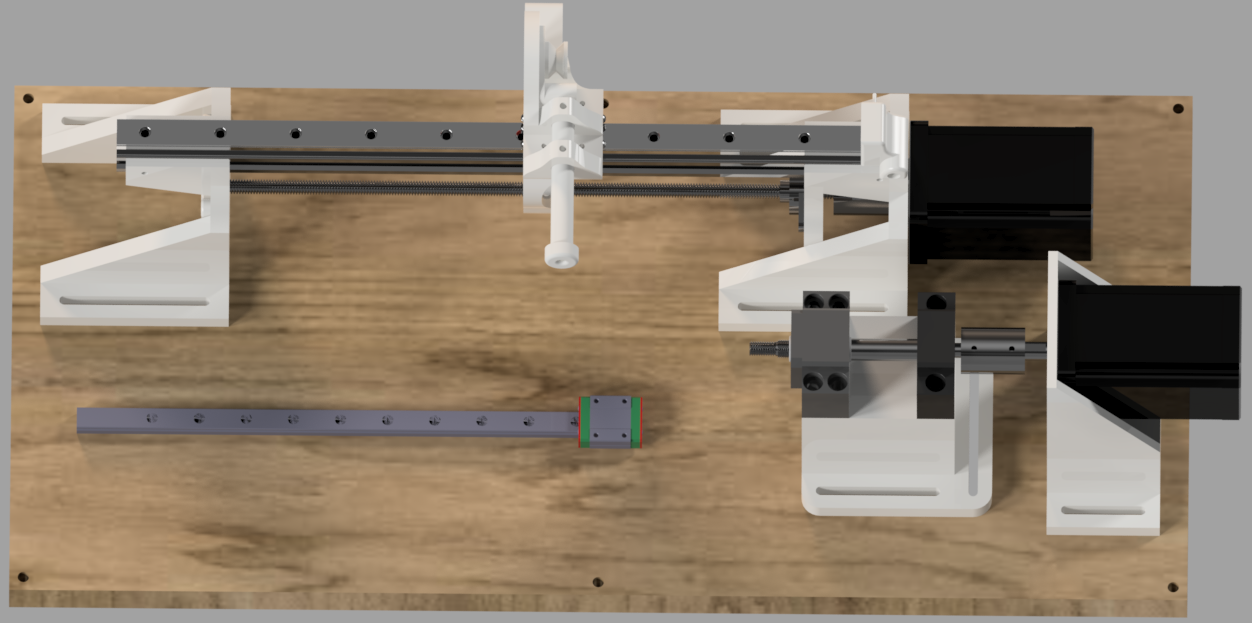
\includegraphics[width=0.25\textwidth]{./winder_render.png}
%     \caption{a nice plot}
%     \label{fig:winder_render}
% \end{figure}



Um einen gleimäßige Wicklung zu gewährleisten, muss die Drahtspannung einstellbar sein und von dieser Idealspannung nur in einem kleinen/bekannten Intervall abweichen. Hierzu wird die Rückstellkraft die auf den Draht wirkt durch zwei Schrauben, welche zwei mit Filz beklebte Platten zusammendrückt, eingestellt. Der Draht wird anschließend durch drei Kugellager geführt, wobei das zweite auf einer Wägezelle montiert ist und die Positionierung so gewählt ist, dass ein- und auslaufender Draht, am Kugellager der Wägezelle, ca. einen Winkel von 180° einschließen. Danach wird der Draht über ein weiteres Kugellager, montiert auf einer, mittels Langloch arritierbaren, Leiste, geführt. Von dort aus läuft er über das letzte Lager, welches am Tänzerarm befestigt ist. Dieser Arm ist kugelgelagert und ca. in der Mitte mit einer Feder verbunden. An dieser Feder ist an ihrem anderen Ende eine Schnur befestigt, welche durch einen Steppermotor aufgewickelt werden kann, um so die Feder zu spannen. Der bewegliche Arm kann somit dynamisch auf Drahtspannugsänderungen reagieren.
